%%%%%%%%%%%%%%%%%%%%%%%%%%%%%%%%%%%%%%%%%%%%%%%%%%%%%%%%%%%%%%%
%
% Welcome to Overleaf --- just edit your LaTeX on the left,
% and we'll compile it for you on the right. If you open the
% 'Share' menu, you can invite other users to edit at the same
% time. See www.overleaf.com/learn for more info. Enjoy!
%
%%%%%%%%%%%%%%%%%%%%%%%%%%%%%%%%%%%%%%%%%%%%%%%%%%%%%%%%%%%%%%%
\documentclass{beamer}

\usetheme{Madrid}
\usecolortheme{lily}
\addtobeamertemplate{footnote}{}{\vspace{2ex}}

\usepackage{amsmath}
\usepackage{amssymb}
\usepackage{color}
\usepackage{listings}
\usepackage{clrscode3e}
\usepackage{multicol}

\definecolor{codegreen}{HTML}{237e02}
\definecolor{codegray}{rgb}{0.5,0.5,0.5}
\definecolor{codepurple}{HTML}{8F4673}
\definecolor{codebrown}{HTML}{ce9178}
\definecolor{codecyan}{HTML}{098658}
\lstdefinestyle{pythonstyle}{
    commentstyle=\color{codegreen},
    keywordstyle=\color{codepurple},
    numberstyle=\tiny\color{codegray},
    stringstyle=\color{codebrown},
    basicstyle=\ttfamily\small,
    breakatwhitespace=false,         
    breaklines=true,                 
    captionpos=b,                    
    keepspaces=true,                 
    numbersep=5pt,                  
    showspaces=false,                
    showstringspaces=false,
    showtabs=false,
    tabsize=2
}
\def\And{\text{ AND }}
\def\Or{\text{ OR }}
\def\Xor{\text{ XOR }}
\def\Implies{\text{ IMPLIES }}
\def\Iff{\text{ IFF }}
\def\Not{\text{NOT}}
\def\R{\mathbb{R}}
\def\N{\mathbb{N}}
\lstset{style=pythonstyle}

\setlength{\parskip}{1em}

%Information to be included in the title page:
\title{Format for Efficient Storage of Homology Relations}
\subtitle{Week 4 Report: Preliminary Experiment Using ETE3 and recPhyloXML}
\author{Kevin Gao}
\institute{University of Toronto}

\begin{document}

\frame{\titlepage}

\AtBeginSection[]
{
    \begin{frame}
    \frametitle{Outlines}
    \tableofcontents[currentsection]
    \end{frame}
}

\section{Parsing XML}

\begin{frame}{ETE Toolkit}
    ETE is an open source Python library for tree analysis.

    \href{http://etetoolkit.org/}{http://etetoolkit.org/}

    The library supports phyloXML and Newick format and provides API for accessing parsed trees: \texttt{ete3.phylo.Phyloxml} and \texttt{ete3.phylo.PhyloxmlTree}.

    The underlying implementation uses \texttt{lxml}, which uses the DOM model, where the entire tree is parsed into the memory, without any caching or indexing.

    Another commonly used package, \texttt{BioPython}, uses \texttt{iterparse()}, which uses a model more similar to SAX (event-based parsing).
\end{frame}

\begin{frame}{GeneTree API}
    We have implemented a set of APIs for parsing and interacting with gene trees encoded in phyloXML format (can be later modified to support recPhyloXML, if needed).
\end{frame}

\begin{frame}{GeneTree API}
    We start from a plain phyloXML file exported from Ensembl Compara. We use the tree ID to query the root node in the mySQL database. The SQL query for obtaining the table is included in the repo.
    \begin{center}
        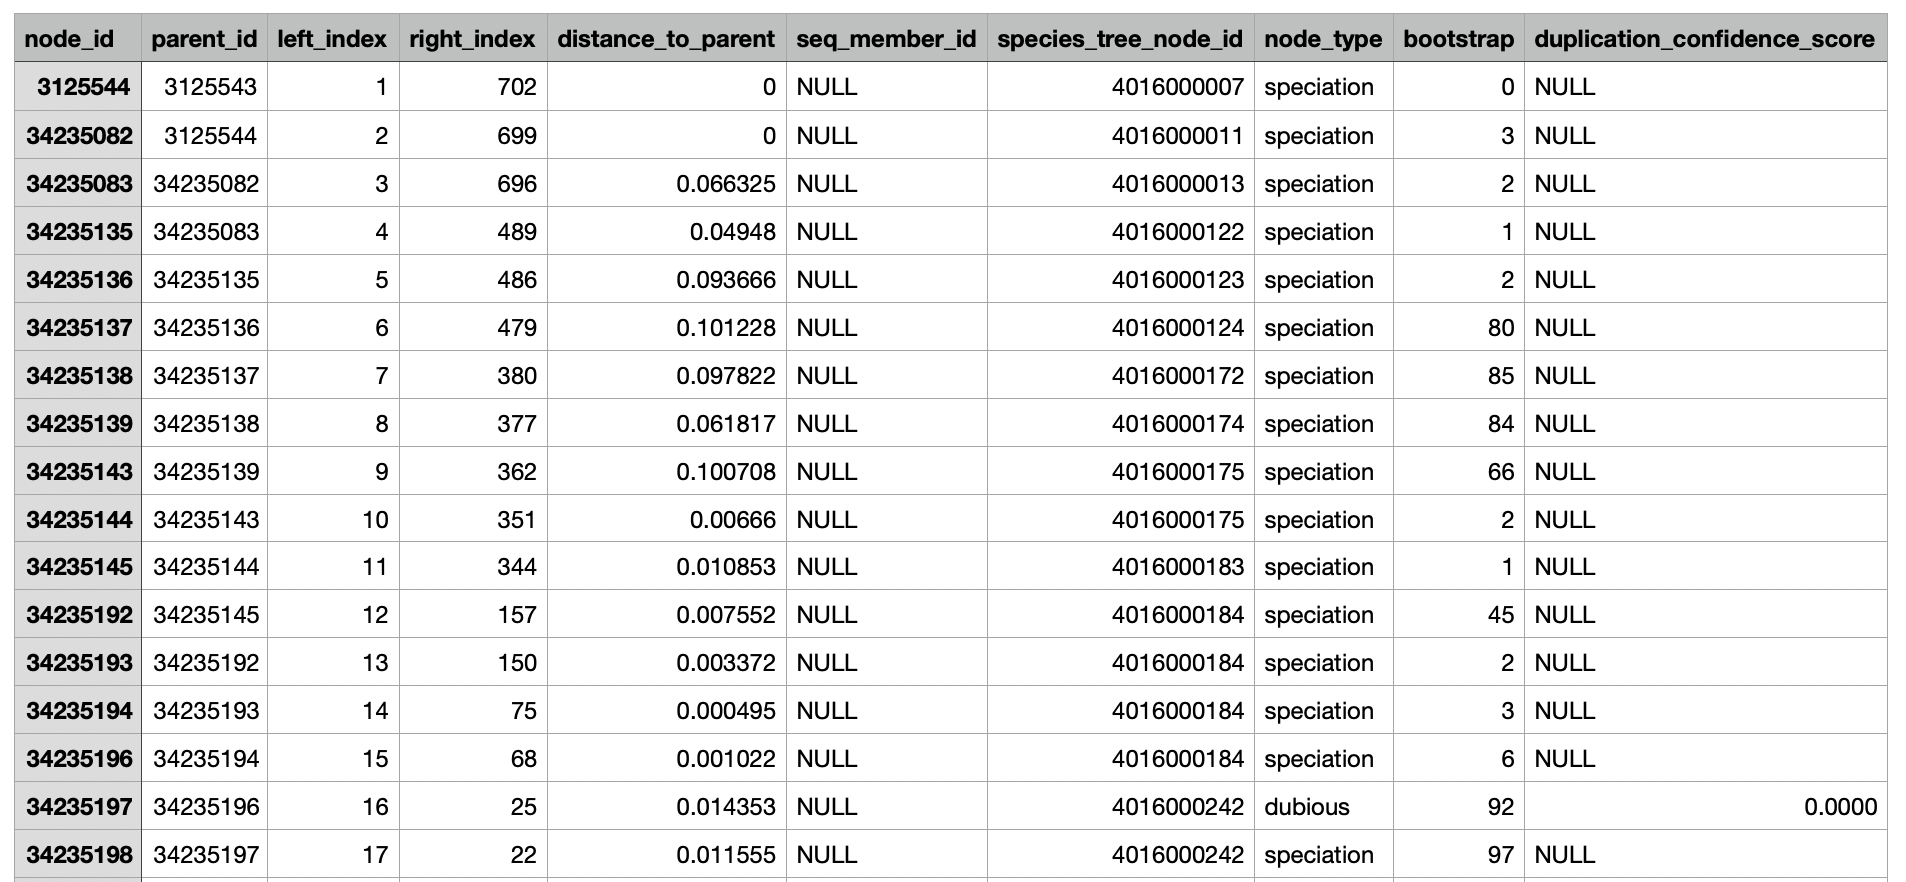
\includegraphics[width=0.9\linewidth]{res/ensembl_db.png}
    \end{center}
\end{frame}

\begin{frame}[fragile]{GeneTree API}
    Once we have the reference table pulled from the database, we can annotate our gene tree (now parsed from phyloXML) to include duplication and speciation events, as well as the confidence score.

    \hfill

    \begin{lstlisting}
gt = GeneTree()
gt.load_phylo_xml('test/test_data/gene_tree.xml')
gt.load_ref_table('test/test_data/ref_table.tsv')
gt.annotate_event_nodes()
    \end{lstlisting}

    Export annotated phyloXML using \texttt{gt.export\_phylo\_xml(..)}.

    Homology inference is done by inspecting the annotation on the lower common ancestor given two leaves.
\end{frame}

\begin{frame}{GeneTree API}
    We plan to include a few benchmark testings for our primitive parser/API implemented in Python using ete. This will be our baseline benchmark. We will compare the result on larger trees with SAX-based parser (especially in terms of memory usage).

    The short-term goal is to implement a phyloXML/recPhyloXML parser using the VTD-XML model with VTD and LC index. However, the library for VTD-XML parser was quite old and was not very well documented. It might take some time to document the parser code and get it to work with phyloXML.
\end{frame}

\section{References}

\begin{frame}
    \scriptsize

    T. C. Lam, J. J. Ding and J. Liu, "XML Document Parsing: Operational and Performance Characteristics," in Computer, vol. 41, no. 9, pp. 30-37, Sept. 2008, doi: 10.1109/MC.2008.403.

    Haim Kaplan, Tova Milo, and Ronen Shabo. 2002. A comparison of labeling schemes for ancestor queries. In Proceedings of the thirteenth annual ACM-SIAM symposium on Discrete algorithms (SODA '02). Society for Industrial and Applied Mathematics, USA, 954-963.

    L. Nakhleh, D. Miranker and F. Barbancon, "Requirements of phylogenetic databases," Third IEEE Symposium on Bioinformatics and Bioengineering, 2003. Proceedings., 2003, pp. 141-148, doi: 10.1109/BIBE.2003.1188940.

    Cardona, G., Rossello, F. and Valiente, G. Extended Newick: it is time for a standard representation of phylogenetic networks. BMC Bioinformatics 9, 532 (2008). https://doi.org/10.1186/1471-2105-9-532

    Kmettlca, E.A. O(log n) persistent online lowest common ancestor search without preprocessing. https://github.com/ekmett/lca/
    
    Wansong Zhang, Daxin Liu and Jian Li, "An encoding scheme for indexing XML data," IEEE International Conference on e-Technology, e-Commerce and e-Service, 2004. EEE '04. 2004, 2004, pp. 525-528, doi: 10.1109/EEE.2004.1287357.
\end{frame}

\end{document}